\subsection{Environment contextualization}\label{sec::desc_contex}

The Jirau plant has horizontal axis bulb type turbines. In hydropower
plants, electric power generation depends on the water level and river flow,
however bulb type turbines are designed just for high water flow to produce
enough electricity. The figure\ref{fig::bulb_turbine} and the
table\ref{tab::bulb_turbine} illustrate a bulb type turbine and the large
ducts needed to hold the large volume of water.
%A usina hidrelétrica de Jirau é do tipo fio d'água, na qual são utilizadas
% turbinas do tipo bulbo de eixo horizontal. Como a geração de energia depende da altura da queda d'água e da vazão do rio, as turbinas do tipo bulbo utilizam uma grande vazão de
%água para produzirem energia elétrica suficiente. A figura
%\ref{fig::bulb_turbine} e a tabela \ref{tab::bulb_turbine} ilustram uma turbina
%do tipo bulbo e o grandes dutos necessários para comportar o grande volume de
% água que passa através da turbina.
 
\begin{figure}[h!]	
	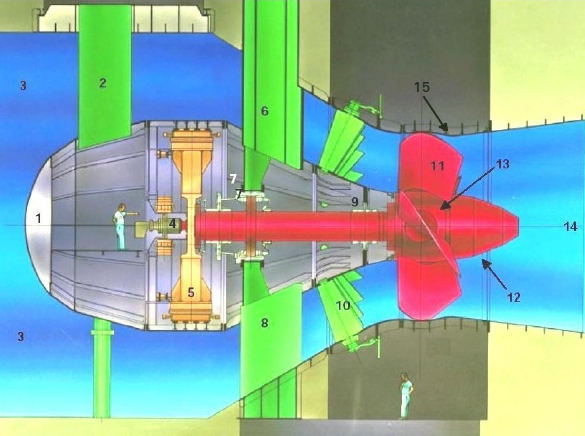
\includegraphics[width=\columnwidth]{figs/intro/bulb_turbine2}
	\caption{Bulb type turbine.}
	\label{fig::bulb_turbine}
\end{figure}

\begin{center}
\begin{tabular}{  c | c  }
  \hline
  \textbf{Number} & \textbf{Name} \\ \hline
  1 & Nose \\ \hline
  2 & Generator access tube  \\ \hline
  3 & Adduction chamber  \\ \hline
  4 & Kaplan head  \\ \hline
  5 & Synchronous generator  \\ \hline
  6 and 8 & Supporting structure \\ \hline
  6 & Turbine access tube \\ \hline
  7 and 9 & Combined bearing and Guide \\ \hline
  10 & Distributor \\ \hline
  11 & Rotor blade \\ \hline
  12 & Cone \\ \hline
  13 & Cube \\ \hline
  14 & Suction tube \\ \hline
  15 & Arc chamber \\
  \hline
\end{tabular}
\captionof{table}{Bulb type turbine principle components}
%\caption{Componentes principais de uma turbina tipo bulbo}
\label{tab::bulb_turbine}
\end{center}

Turbine repair or inspection requires water flow stoppage and water drainage. In
Jirau, there is a 80 cm diameter access (hatch) for rotor maintenance. In the
context of the proposed solution, the turbine points of interest are:

%Atualmente, caso seja necessário algum reparo ou inspeção na turbina, é
% necessário que se interrompa o fluxo de água e que toda a água em seu interior seja drenada. Para manutenção do rotor, existe uma escotilha de acesso de diâmetro limitado. Entretanto, caso deseje-se realizar 
%a metalização de pás já instaladas, utilizando-se os processos atuais, é
%necessária a retirada de todo o aro câmara, desmontagem completa do rotor e
% logística de transporte das pás até o local onde a metalização será realizada. Essa operação, caso necessite ser realizada, demandaria a mobilização
%de diversas equipes de manutenção, operação de pórtico rolante e transporte,
%além de impossibilitar a utilização da turbina durante várias semanas.
%No contexto da solução proposta, os pontos de interesse da turbina são:

\begin{itemize}
  \item propeller and blades;
  \item Ring chamber and adjacent areas;
  \item Hatcher of access;
  \item Suction tube;
  \item Available infrastructure.
\end{itemize} 

\subsubsection{Propeller and blades}
 
The rotor or turbine propeller consists of the hub, the blades and the cone.
Blades of Jirau turbine measure approximately 2.5 m tall and
3 m wide, they are fully reachable from the turbine interior,
excepting edges and lips, which can be visualized through a small top hatch
access. The figure\ref{fig::blade_rijeza} exemplifies a turbine blade recently
coated by Rijeza company. 
%O rotor ou hélice da turbina é constituído do cubo, as pás e o cone. 
%Nas turbinas da usina de Jirau, cada pá mede, aproximadamente, 2,5m de altura e
%3m de largura. A partir do interior da turbina, todas as superfícies da pá são
%alcançáveis, com exceção da borda e do lip da pá. O único ponto de acesso à
%essa regiâo é por meio da escotilha superior de acesso. A figura
%\ref{fig::blade_rijeza} exemplifica uma pá do rotor presente na usina de Jirau
% recém metalizada no galpão da Rijeza.

\begin{figure}[h!]	
	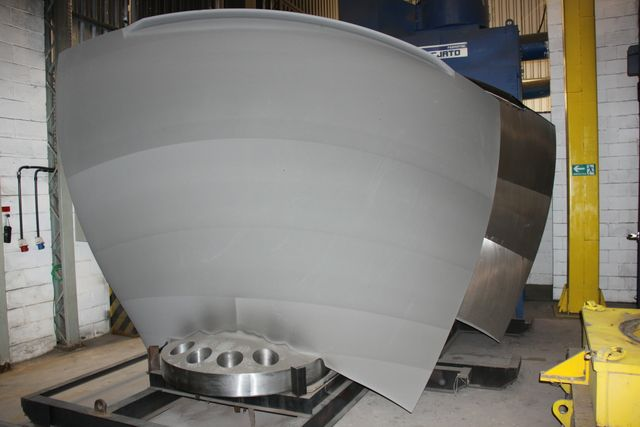
\includegraphics[width=\columnwidth]{figs/viagem/2015_04_28/Rijeza/img_4887}
	\caption{Jirau turbine blade.}
	\label{fig::blade_rijeza}
\end{figure}


The blades angles relative to the water flow can be changed $\pm 14.5$ from the
starting position, without overlapping areas, figure
\ref{fig::blades_angle}. These angles can be exploited to optimize working space
for blade coating process and also influences the working region between
the distributor and the rotor. Blades angles and rotor position can be changed
manually, and the last could be rotated in both directions without limit.
However, this operation is an imprecise and risky task. Hence, the proposed
solution should optimize rotations required for the blade processing.
%A angulação de cada pá em relação ao fluxo d'água pode ser alterado em 29$^o$,
%14.5$^o$ para cada lado a partir da posição inicial, não havendo sobreposição
%entre as pás, como ilustrado na figura \ref{fig::blades_angle}.
%Essa angulação pode ser explorada para otimizar o espaço de trabalho necessário
%para o processamento da pá e também influencia o acesso à região
%entre o distribuidor e o rotor, uma vez que não existe acesso pela montante da
%turbina. Entretanto, vale observar que esta angulação não pode ser alterada
%manualmente e só pode ser realizada uma vez, antes do desligamento da turbina.
% A posição do rotor também pode ser manualmente alterada, possibilitando que o
%mesmo seja girado em ambas as direções e sem limite de revoluções. Entretanto,
%essa operação é uma tarefa imprecisa e envolve um certo risco às pessoas que a
%realizam. Sendo assim, a solução proposta deve otimizar o número de rotações
%necessárias para o processamento de todas as pás.

\begin{figure}[h!]	
	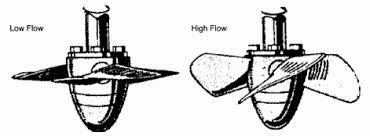
\includegraphics[width=\columnwidth]{figs/intro/blades_angle}
	\caption{Example of the blade angle limits.}
	\label{fig::blades_angle}
\end{figure}

\subsubsection{Ring chamber and adjacent regions}

The arc chamber, as the distributor area and the suction tube, has metal
surface. This characteristic allows magnetic fixing solutions for robotic
systems. However, the cylindrical and sloping shape of aro camara, and the
turbine distributor hinder robot fixation and movement. An horizontal plane or
an efficient and robust base should be build for the system fixation.
Under turbine maitenance, devices and equipments are fixed by scaffolding
anchored by ropes. The figure~\ref{fig::andaime} illustrates a turbine under
maintenance.
%O aro câmara, assim como o a região próxima ao distribuidor e também ao tubo de
%sucção possuem superfícies metálicas. Essa característica possibilita a
%exploração de soluções de fixação magnética.

%Somente a região compreendida pelo aro câmara é plana e tendo como agravante a
% presença do distribuidor na região à montante ao rotor. É necessário que a inclinação presente nessas superfícies seja contabilizada e uma solução eficiente 
%de apoio ou plano elevado seja desenvolvida caso haja necessidade de fixação de
% alguma parte do sistema. Atualmente todo o trabalho é realizado por meio da montagem de andaimes ancorados por cordas. A
%figura \ref{fig::andaime} ilustra uma estrutura utilizada no modo de inspeção e
%manutenção atuais.

\begin{figure}[h!]	
	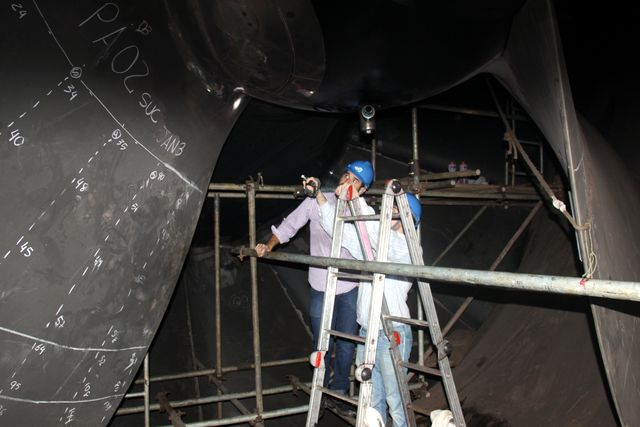
\includegraphics[width=\columnwidth]{figs/viagem/2015_04_28/UG/img_4969}
	\caption{Turbine under maintenance. Scaffolding as fixation points for
	equipments.}
	\label{fig::andaime}
\end{figure}

 
\subsubsection{Hatches}
The turbine accesses are two hatches: the bottom hatch is located at the
beginning of the suction tube, next to the ring chamber; and the top hatch is
located at the top of the ring chamber.
%O acesso à turbina se dá por duas escotilhas, uma inferior, localizada no
% ínicio do tubo de sucção próxima ao aro câmara e outra superior, localizada na parte superior do aro câmara.

Operators access the turbine via the bottom hatch and all equipments for
maintenance are transported through this hatch. The bottom hatch diameter is
80 cm.
%A escotilha inferior é o acesso utilizado para a entrada de pessoas na turbina
% e todo material utilizado para reparos é transportado através dessa escotilha. Na usina de Jirau existem dois 
%tipos de escotilha de acesso inferior, sendo a menor delas possuindo 80cm de
% diâmetro.

The top hatch is used mainly for blade lip visual condition inspection. The
diameter of the top access is approximately $35.7cm$, thus no equipments
are transported through this hatch. The figures~\ref{fig::esc_sup_ext} e
~\ref{fig::esc_sup_int} illustrate the top hatch from different views.
%A escotilha superior é utilizada, principalmente, para a inspeção visual do
%estado dos Lips das pás.
%O diâmetro do acesso superior é de aproximadamente $35.7cm$, limitando as
%dimensões dos equipamentos que podem ser transportados através da escotilha. As
% figuras \ref{fig::esc_sup_ext} e \ref{fig::esc_sup_int} ilustram o acesso à escotilha superior pelo exterior ao
%aro câmara e a visão pelo interior da turbina,
%respectivamente.

\begin{figure}[h!]	
	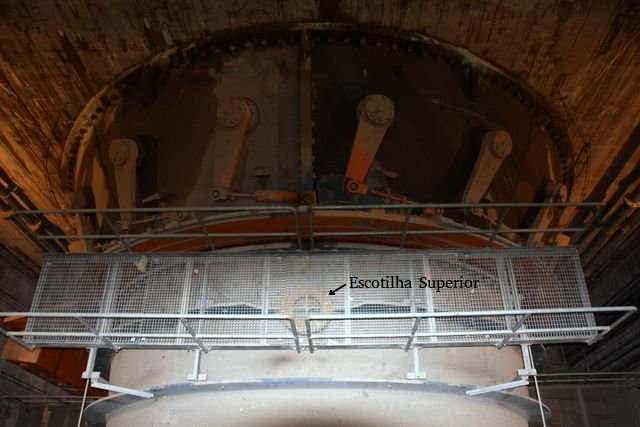
\includegraphics[width=\columnwidth]{figs/viagem/2015_04_28/UG/img_4979_mod}
	\caption{Top hatch view - ring chamber exterior}
	\label{fig::esc_sup_ext}
\end{figure}

\begin{figure}[h!]	
	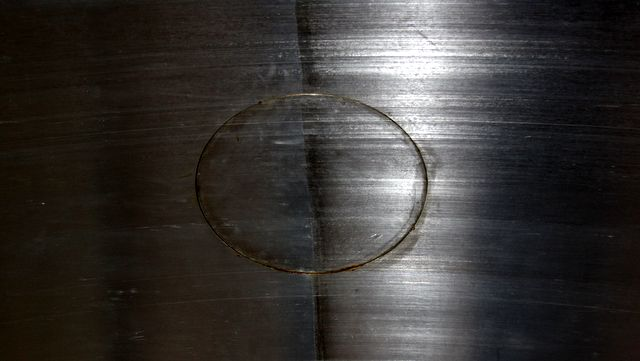
\includegraphics[width=\columnwidth]{figs/viagem/2015_04_28/UG/img_4982}
	\caption{Top hatch view - ring chamber interior}
	\label{fig::esc_sup_int}
\end{figure}

\subsubsection{Suction tube}

At the end of the discharge pipe is located the downstream stoplogs and then the
riverbed. If the stoplog are not inserted, there is a 10 m wide gap, which
could be used as access. However, the high water flow due to the
openning of the distributor make it impossible for access. The distributor is
not closed immediately due to environmental issues, since this becomes the
passage of fish.
%Ao final do tubo de descarga está localizado o vão dos stoplogs 
%de jusante ou da comporta vagão e, em seguida, o leito do rio. Caso os stoplogs 
%não estejam inseridos, existe um vão de, pelo menos, 10 m de largura. Porém,
% não é válida a utilização deste vão como acesso à turbina, pois há grande fluxo de
%água devido à abertura do distribuidor. O distribuidor não é fechado
%imediatamente por questões ambientais, já que este é o escoamento de peixes.

%criando assim
%um acesso extra para um sistema submarino. A figura \ref{fig::tubo_suc}
%exemplifica a magnitude do tamanho do acesso, deixando claro que o limitante de
%tamanho do sistema para a utilização desse acesso é o vão de entrada do
% stoplog, ilustrado na figura \ref{fig::stoplog}. Outra alternativa é utilizar um
%guindaste e submergir o sistema pelo próprio rio, entretanto o sistema ficaria
%sujeito as condições do ambiente.

\begin{figure}[H]	
	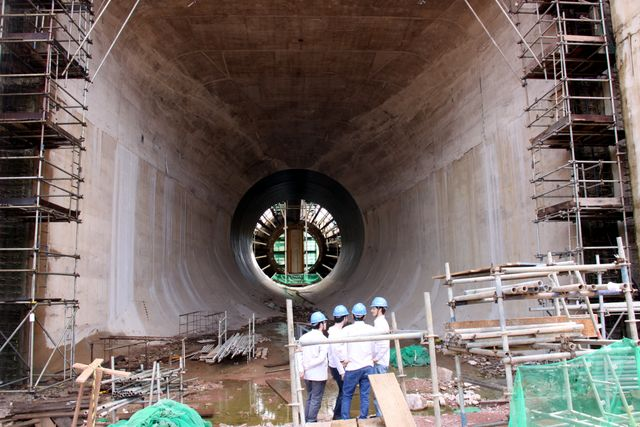
\includegraphics[width=\columnwidth]{figs/viagem/2015_04_30/Vao/img_5086}
	\caption{Suction tube openning under construction.}
	\label{fig::tubo_suc}
\end{figure}

\subsubsection{Available infrastructure}
After the turbine drainage, maintenance provides electricity and compressed
air, requirements for the HVOF process. Other important factor is the presence
of a gantry crane outside the turbine, but could position the HVOF necessary
equipment nearby the top hatch. Also, it is possible to access the top hatch
through the gantry crane.
%É importante ressaltar a infraestrutura dísponível para o desenvolvimento da
% solução.
%Após secar a turbina, é possível a disponibilização de energia elétrica e ar
%comprimo em seu interior, ambos importantes para o processo de metalização.
% Outro fator importante é a presença de um pórtico rolante que tem acesso até o andar diretamente 
%inferior ao aro câmara, posicionando todo o equipamento necessário nas
% proximidades da escotilha de acesso inferior. É possível também o acesso direto, por meio de pórtico, 
%à escotilha superior.

\begin{figure}[h!]	
	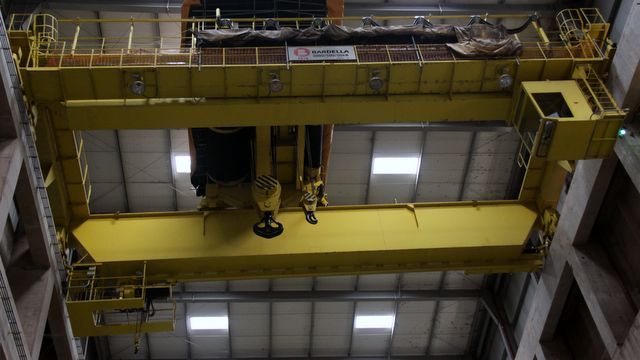
\includegraphics[width=\columnwidth]{figs/viagem/2015_04_28/UG/img_4989}
	\caption{Gantry crane and top hatch}
	\label{fig::portico}
\end{figure}

The environment may be briefly characterized by the blades dimensions,
element to coated; the ring chamber structure, which limits
the workspace of the robot; and the access.
%O ambiente pode ser resumidamente caracterizado pelas dimensões das pás,
%elemento a ser processado; características do aro câmara, estrutura que limita
% o espaço de trabalho do robô; e pelos acessos nos quais o sistema terá que
%utilizar.

\begin{itemize}
  \item \textbf{Turbine blades} - 420 stainless steel. Dimensions 2.5 x 2.5 m;
  \item \textbf{Ring chamber} - cylindrical structure 3.95 radius and metal
  surface;
  \item \textbf{Access}: 
  	\begin{itemize}
    	\item Top hatch - 35 cm diameter;
  		\item Bottom hatch - 80 cm diameter;
  		\item Suction tube - 20 x 20 m, access by river. 
  	\end{itemize}
\end{itemize}

A 3D CAD model of the turbine was built in SolidWorks for
conceptual solution analysis and future simulation
(figura~\ref{fig::ambiente3d}). The model is not fully detailed, but the
upstream tunnel, the stator, the rotor, a small sector of the downstream, and
the hatches are represented with great accuracy.
%Os estudos das possíveis soluções exigiu uma visualização mais detalhada do
%volume livre no interior da turbina. Para isso, foi recriado o ambiente da
%turbina em CAD 3D no SolidWorks, a partir dos desenhos 2D de seção da turbina
%fornecidos pelo cliente.
%O modelo tridimensional do aro câmara permite o estudo e o dimensionamento
%% geométrico de alcance do manipulador para cada solução. Não foram necessários
%detalhamentos de todos os componentes, podendo ser apenas considerados, e
%representados com maior precisão, os perfis externos do túnel à montante, o
%estator, o rotor e uma pequena região à jusante, além dos acessos
%por escotilha superior e inferior.
%A figura~\ref{fig::ambiente3d} apresenta o ambiente da turbina em CAD e os
%possíveis acessos para realização das intervenções.

\begin{figure}[h!]
\centering
	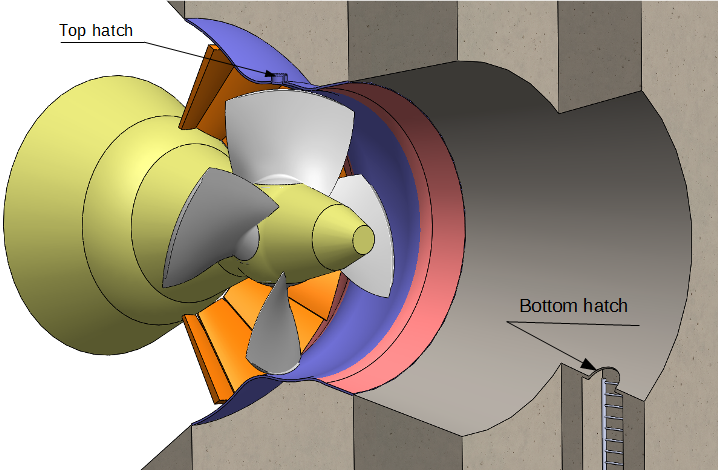
\includegraphics[width=\columnwidth]{figs/estudo/solid/ambiente_3d} 
	\caption{3D CAD model of the Jirau turbine (SolidWorks)}
	\label{fig::ambiente3d}
\end{figure}




